\chapter{Background Literature}\label{ch:lit}

\section{An imperative to engage}\label{sec:litspi}

%\textcite{vonSchneidemesserMS2020} reframe it as a system

A dominant conceptualisation of the interactions of science and public policy is the \SPI{} (\cite{JagannathanEtAl2023}). This interface represents the institutions and mechanisms by which knowledge is transferred between the processes of scientific enquiry and public policy decisionmaking. In its traditional form, \emph{the rational model}, evidence derived from scientific enquiry is used to inform policy decisions and thus science is often considered to \emph{supply} knowledge in response to \emph{demand} from policy. In reality, the \SPI{} a ``complicated and erratic flow of information'' (\cite{BednarekSHG2015}) that is constantly evolving with changing values, demands and understanding of science, policy and society (\cite{Obermeister2020}). Yet, despite being ``widely debunked'' (\cite{BoswellS2017}, also \cite{McNie2007,HaynesDCRHGS2011,Cairney2018}), the rational supply-demand model persists implicitly in much literature about the \SPI, resulting in normative guidance for scientists to align their actions better with the needs of policy (e.g. \cite{McNie2007,GeddesDP2018,BlessenohlS2022,Bisbal2024}).

Such guidances, and their underlying research and discussion, are well-intended efforts to close the ``gap'' that is widely recognised between science knowledge and policy goals (e.g. \cite{RapleyD2014,KarlssonG2020,CairneyTS2023}). Some of the greatest consequences of this gap is the delay in policy, and thus action, related to the worsening \CAN{} crises. These intersecting crises of a destabilising climate (\cite{IIPCC2022}) and deteriorating nature (\cite{IPBES2022}) and are already threatening and undermining the lives and livelihoods of people in a myriad of guises (\cite{TschakertEAKO2019,SpaiserEtAl2024}) and the implications for humanity as a whole are dire (\cite{McKayEtAl2022,WEF2024,SpaiserEtAl2024}). The disputes and uncertainties of \CAN{} science, coupled with the urgency and high stakes of \CAN{} policy has been characterised as \PNS, requiring new approaches to decision-making incorporating a complexity of knowledges, known as \emph{extended peer review} (\cite{FuntowiczR1993,Ravetz1999,Jasanoff2003}). Yet, while policymakers have changed their perspectives on these issues a great deal (\cite[p118]{Killick2023}), there has been a failure recognise and respond to the unstructured and emergent nature of \CAN{} issues (\cite{FuntowiczR1993,WesselinkH2020}), which instead are ``tacked onto how they always thought about the economy'' (\cite[p118]{Killick2023}). The gap here is lack of policy that is commensurate with the scale and urgency of the \CAN{} crises. Rather than construing the gap as an issue of the misalignment of scientists to policy, the implication is that it is a misalignment of the \SPI{} to the \CAN{} crises (\cite{BalvaneraJNOBCDGGKKMPSSW2020}).

%This has not gone unnoticed, \SPI{} boundary organisations have been established worldwide within which scientists engage directly on science-related policy (\cite{WesselinkH2020}), including international bodies such as the Intergovernmental Panel on Climate Change, Intergovernmental Science-Policy Platform on Biodiversity and Ecosystem Services, Climate Change Committee and Joint Nature Conservation Committee. 
%For instance the \IPCC{} and the \IPBES{} are international organisations tasked with establishing policy-relevant science, drawing on wider knowledges and values (e.g. \cite{PascualEtAl2018,MatukBSAHT2020})  and producing the policy advice. Policy itself is made nationally and locally, requiring the relevant knowledge to be convened in these contexts. In the UK, the \CCC{} is the independent statutory body for advising the UK and devolved governments on climate-related policy and the \JNCC{} is the statutory nature adviser for UK and devolved governments. Outside of boundary organisations, 

\section{Roles at the science-policy interface}\label{sec:litroles}

Many researchers studying the processes, practices and pathways by which knowledge meaningfully informs policy, consider that \SPI s need prescribed intermediaries between scientists and policymakers (\cite{JagannathanEtAl2023}). Thus, a number of boundary-spanning roles are defined within the theoretical literature, summarised in Table~\ref{tab:litroles}. These roles embody different values, objectives and strategies for knowledge creation and exchange with policymaking, but largely imply a one-way transfer of knowledge, as exemplified by \textcite{SteelLLS2004}'s \emph{reporting}, \emph{interpreting}, \emph{integrating}. The work of Roger A. Pielke, Jr. has been highly influential in describing an idealised set of roles at the \SPI: \emph{Pure Scientist}, \emph{Science Arbiter}, \emph{Issue Advocate} and \emph{Honest Broker of Policy Alternatives} (\cite{Pielke2007}), with emphasis on the scientist's credibility and the science's legitimacy (\cite{DuncanRE2020}). This set of roles has been developed both over recent years (e.g. \cite{RapleyD2014,DuncanRE2020,GluckmanBK2021,GregoryBW2024}). %The table also includes a summary of a further role, the \emph{Policy Entrepreneur}, probably the best known policy intermediary, although not necessarily one that interfaces with science.

\begin{table}[!ht]
\footnotesize
\caption{Roles of relevance to the \SPI}\label{tab:litroles}
\begin{tabular}{L{.48\linewidth}L{.30\linewidth}L{.22\linewidth}}  \hline
\textbf{description} & \textbf{similar roles} & \textbf{empirical examples} \\ \hline \hline
\multicolumn{3}{c}{\textbf{\small Pure Scientist}} \\ 
Generates and shares knowledge and without consideration for its use (\cite{Pielke2007,RapleyD2014}) & Knowledge Generator (\cite{BalvaneraJNOBCDGGKKMPSSW2020}) & \textcite{SteelLLS2004,SinghTKMMC2014} \\ \hline
\multicolumn{3}{c}{\textbf{\small Science Communicator}} \\ 
Engages with society offering expert interpretation and drawing attention to the implications (\cite{RapleyD2014}) & Interpreting (\cite{SteelLLS2004}) & \textcite{SteelLLS2004,SinghTKMMC2014} \\ \hline
\multicolumn{3}{c}{\textbf{\small Science Arbiter}} \\ 
Using scientific findings to answer questions that the policymaker thinks are relevant without expressing opinion (\cite{Pielke2007,GluckmanBK2021}) & Synthesiser (\cite{KarkkainenLKK2024}) &  \\ \hline
\multicolumn{3}{c}{\textbf{\small Science Adviser}} \\ 
Scientists called on to synthesise the existing science and interpret it for the policy context. \textcite{Obermeister2020} describes how this role is a process of learning and becoming increasingly expert and thus can be considered the transition between Science Arbiter and Knowledge Broker (\cite{Obermeister2020,GluckmanBK2021}) & Interpreting (\cite{SteelLLS2004}) & \textcite{SteelLLS2004,SinghTKMMC2014,Obermeister2020} \\ \hline
\multicolumn{3}{c}{\textbf{\small Knowledge Broker}} \\ 
Translates knowledge to the given setting, communicates it across disciplines (\cite{GogginEtAl2015}) contributing their own expertise (\cite{RapleyD2014}), including knowledges other than those of science and policy (\cite{Gluckman2014}) & Honest Broker of Policy Alternatives (\cite{Pielke2007}) Commentator (\cite{KarkkainenLKK2024}) Integrating (\cite{SteelLLS2004}) & \textcite{SteelLLS2004,SinghTKMMC2014,BednarekSHG2015} \\ \hline
\multicolumn{3}{c}{\textbf{\small Advocate}} \\ 
Advocate for attention to be paid to a particular cause (\cite{KarkkainenLKK2024}). Scientists with expert knowledge about the cause may use advocacy depending on their values (\cite{RykielEtAl2002,RapleyD2014,ElsensohnACDGGKPRS2019}).  & Issue Advocate (\cite{Pielke2007}) Policy Advocate (\cite{ScottRLPAFSRSS2007}) Taking a Position (\cite{SteelLLS2004}) Honest Advocate (\cite{RoseBOP2018,GregoryBW2024}) %Stealth Advocate (\cite{Pielke2007})
& \textcite{SteelLLS2004,ScottRLPAFSRSS2007,SinghTKMMC2014,RoseBOP2018,DablanderSCSBGGBAH2024} \\ \hline
%\multicolumn{3}{c}{\textbf{\PE}} \\ 
%Focused on influencing policy using a range of means (\cite{Kingdon1993}) that are not necessarily derived from objective evidence, raising questions of legitimacy, accountability, justice (\cite{vonMalmborg2024strategies}). Therefore, this is not recommended for scientists but of relevance to scientists because of their presence at the \SPI. & Problem Broker (\cite{Knaggard2015}) Interpretive Policy Entrepreneur (\cite{AukesLB2018}) & \textcite{CarterC2018} (Friends of the Earth as a \PE) \textcite{MintromL2017} (\PE s in climate policy)  \\
%\hline
\end{tabular}
\end{table}

These roles are not without major dilemmas (\cite{CairneyO2020}). As will be seen in the next section, advice to scientists about \SPI{} engagement includes a recommendation to choose between advocacy and advice/brokerage (\cite{OliverC2019}) or to avoid advocacy altogether (\cite{Gluckman2014}). This is an ongoing debate about the impacts of advocacy on the trust in, and the credibility of, science and scientists (\cite{Edwards2013,GregoryBW2024,ColognaKMBMO2024,DablanderSCSBGGBAH2024,RykielEtAl2002}), although there is increasing evidence of the involvement of \CAN{} scientists in a range of advocacy activities (\cite{ColognaKMBMO2024,DablanderSCSBGGBAH2024,ScottRLPAFSRSS2007}). Even when avoiding advocacy, adviser and brokers can experience tensions between the ``sacred'' objectivity of science and the ``profane'' of co-producing solutions (\cite{WesselinkH2020,MacKillopCDD2023}) and reconciling the disputed and uncertain scientific knowledge with the desire of policy for consensus and certainty (\cite{Stirling2010,Hicks2024}). This is not simply frustrating, the reputations of scientists, and science itself, can be damaged when nuance is insufficiently communicated (\cite{Stirling2010,OjanenBKP2021}).

%To some, advocacy, whether for an issue or a particular policy, is seen by some as undermining the credibility of science, or at least the scientist (\cite{Edwards2013}). \citeauthor{Pielke2007} warned about the \emph{Stealth Advocate} who uses their credibility as a scientist to argue for a particular cause, even when the science is not settled (\cite{CardouV2023,GluckmanBK2021}). However, others have argued that the urgency and scale of our \CAN{} challenges are trivialised when scientists do not take a strong position on political action (\cite{GregoryBW2024}). The choice to advocate is often left to individual scientists to make based on their own values (\cite{RykielEtAl2002}). A survey by \textcite{DablanderSCSBGGBAH2024} and a narrative review by \textcite{ColognaKMBMO2024} both find that there are nuances to the affect on trust in science and scientists of their advocacy that depend on what is being advocated for, and the audience perceiving the advocacy. Significantly, both papers note the engagement of thousands of scientists in some aspect of climate campaigning, and a review of 270 conservation articles identified that policy advocacy was present in almost all of them (\cite{ScottRLPAFSRSS2007}).  

%Even choosing advice or brokerage can create tensions. \textcite{WesselinkH2020} contrasts the ``sacred'' objectivity of science with the ``profane'' of co-producing solutions. Empirical evidence points to scientists experiencing pressure to produce evidence that aligns with a particular policy perspective (\cite{MacKillopCDD2023}) and personal accounts from science advisers articulate tensions between the desire of policymakers for certainty and consensus, and the disputed and uncertain nature of scientific knowledge  (\cite{Stirling2010,Hicks2024}). Such pluralities of perspective may be difficult to reconcile in policy settings that demand communications in a condensed form. This is not simply frustrating, the reputations of scientists, and science itself, can be damaged when nuance is insufficiently communicated (\cite{Stirling2010,OjanenBKP2021}). The work of producing scientific evidence is held to a rigorous set of values that are in tension with the ``moral and political framework'' into which this evidence is submitted (\cite{Nau2009}, quoting \cite[p263]{Bull1972}).

\section{Practices at the science-policy interface}\label{sec:litpractices}

The evidence is that scientists are not confident about engaging with policy (\cite{KEU2021perceptions}), despite their input being recognised at ``vital'' (\cite{KennyRHTB2017}). Accordingly, governmental policymaking functions have produced a range of documents that define and describe principles and practices of science-policy intermediation (e.g. \cite{OECD2015,DottiACDMPSVW2024,KarkkainenLKK2024}). There is also a great body of Policy Studies literature theorising the behaviours of individuals, groups and processes in policymaking (e.g. \cite{Kingdon1993,Hajer2005,Dowding2018}), with \textcite{KernR2018} performing an excellent analysis of how the main 5 theories in this literature apply to sustainability transitions. This literature provides theories about practices that improve outcomes of engagement at the \SPI{} (e.g. \cite{RykielEtAl2002,McNie2007,Gluckman2014,BlessenohlS2022}). However, this is not widely used in research into climate justice policy (\cite{CairneyTS2023}) and empirical evidence about the use and success of practices a the \SPI{} is harder to come by (\cite{JagannathanEtAl2023}). \textcite{OliverHBGC2022} review the empirical evidence of how research impacts policy, but find it lacks rigour. Combining the Policy Studies theoretical and empirical literatures, along with `how to' advice, \textcite{OliverC2019} synthesised 8 tips for influencing policy, summarised in Table~\ref{tab:litpractices}.

\begin{table}[!ht]
\footnotesize
\caption{Tips for engaging at the \SPI{} after \textcite{OliverC2019}, with some examples of where they have been empirically observed}\label{tab:litpractices}
%\begin{tabular}{L{.22\linewidth}L{.56\linewidth}L{.22\linewidth}} 
\begin{tabular}{L{.68\linewidth}L{.32\linewidth}} \hline
\textbf{description} & \textbf{empirical examples}\\ \hline \hline
\multicolumn{2}{c}{\textbf{\small Do high quality research}} \\
Research should be relevant to policy and rigorously performed, determining uncertainties, strengths and weaknesses. 	 & 	\textcite{RoseBOP2018,OjanenBKP2021,IbarraJOBCIMRS2022} \\ \hline
\multicolumn{2}{c}{\textbf{\small Effectively communicate research}} \\
Policymakers need research communicated in ways that are credible, accessible and meaningful, such as by \emph{framing} research in terms of a particular policy priority. & 	\textcite{RoseBOP2018,Obermeister2022} \\ \hline
\multicolumn{2}{c}{\textbf{\small Understand policy processes}} \\
Policymaking is non-linear and dynamic, with diverse structures and authorities. Evidence needs to be translated for each context.	 & 	\textcite{Obermeister2022} \\ \hline
\multicolumn{2}{c}{\textbf{\small Be accessible to policymakers}} \\
Scientific advice is often required at specific times to address specific questions	 & 	\textcite{GogginEtAl2015} \\ \hline
\multicolumn{2}{c}{\textbf{\small Decide if you want to be an issue advocate or honest broker}} \\
Many commentators find the two roles incompatible with each other and recommend being open about advocating for particular causes. & \textcite{ScottRLPAFSRSS2007}\\ \hline
\multicolumn{2}{c}{\textbf{\small Build relationships with policymakers}} \\
Engagements with will often arise through network connections and trust and shared understandings are essential under pressurised situations but take time and effort to develop.	 & 	\textcite{OjanenBKP2021,IbarraJOBCIMRS2022,SaxonbergSL2023} \\ \hline
\multicolumn{2}{c}{\textbf{\small Be `entrepreneurial' or find someone who is}} \\
The opportunities to establishing new relationships and engage with policymakers may be unusual or fleeting, suggesting a need to be ready when a \emph{Window of Opportunity} opens. This may be too much effort for an individual scientist and collaboration with others is recommended.	 & 	\textcite{RoseBOP2018} \\ \hline
\multicolumn{2}{c}{\textbf{\small Reflect continuously}} \\
The science-policy and personal contexts require different approaches and decisions on whether to engage. & 	\textcite{OjanenBKP2021,Obermeister2022} \\
\hline
\end{tabular}
\end{table}

These 8 tips for engaging reflect policy perspectives, such as \emph{Problem Framing}, which is used define an nature of and issue and thus determine the relevant domains of knowledge (\cite{OECD2015,MoallemiZHSMZHKHMGLB2023}), and \emph{Windows of Opportunity} (\cite{Kingdon1993}), when it may be possible to cast new ideas into the policy arena (\cite{RoseBOP2018}). The 8 tips also reflect the observation that advice to scientists is to conform to the policymaking process. As such, many of these are ``safe solutions'' that belie several tensions experienced by those engaging with policy (\cite{CairneyO2020}) such as the how political context (\cite{SaxonbergSL2023,WesselinkH2020}) and power imbalances (\cite{TurnhoutMWKL2020,OjanenBKP2021,StrassheimK2014}) shape what knowledge may or may not be admissable; the pressure to censor in order to remain admissable (\cite{Pearce2024,OjanenBKP2021}); and, particular to the natural sciences, the aversion to raising ``false alarms'' (\cite{ReadO2017,PoeS2023}) which may instead underplay the implications of \CAN{} scientific findings (\cite{CalverleyA2022}). 

\section{Influencing at the science-policy interface}\label{sec:litinfluencing}

The discipline of Policy Studies is beginning to recognise that Behavioural Science has much to offer in insights into how decisions are made and how to influence them (\cite{CairneyW2017}). \textcite{Darnton2008} provides a detailed resource that brings together a multitude of behaviour change models (alongside theories of change). However, such insights into the influences on, and responses of, individuals are largely focused on the behaviour of individuals and society and is thought of as informing the design of behaviour change policy,  less so informing the policymaking process itself, which is a curious oversight. Instead, decisions in policymaking are predominantly referred to as using \emph{Bounded Rationality} (\cite{CairneyO2020,CairneyTS2023}), an economic model of decision-making, which considers that satisficing, rather than optimising, choices are made based on the available information. 

Indeed, the underlying model behind advice on influencing policymakers supposes that they are deficient in relevant information. This is not dissimilar to the so-called the \IDM{}, the idea that better decisions on science topics would be made if people better science information. The \IDM{} has unknown origins (\cite{Nerlich2017}) and may simply be an intuitive response: ``if they knew what I know, they'd behave differently''. However, a number of related models have been developed based on ideas of information deficit (\cite{Darnton2008}). The \IDM{} prompts a strategy of communicating more information. This has been more formalised regarding \CAN{} issues as the Gateway Belief Model, through which \textcite{vanderLindenLFM2015} and \textcite{vanderLinden2021} posit that communicating scientific consensus on climate change will alter attitudes to the issue. Whilst the \IDM{} has largely been shown to have only short-term relevance (\cite[p24-5]{BA2024trust}), the intuition that more information is what is needed to create change will continue to motivate knowledge sharing strategies.

Moving beyond models of information deficit, Behavioural Science and Environmental Psychology propose a wide range of models to describe what motivates and constrains people's behaviours (\cite{Darnton2008}). Recent efforts have created compilations of behaviour change models, with a particular aim to support the social transitions required to address \CAN{} issues (thus, still not specifically about policy decision-making). These include the \ISM{} (\cite{DarntonH2013}, based on \cite{SouthertonME2011}; Figure~\ref{fig:ism}), which divides influences into the individual, social, and material, the Theoretical Domains Framework (\cite{AtkinsFIOPIFDCGLM2017}), which has 14 clusters of behaviour change theories, and the model of \textcite{HamptonW2023} which brings together individual, social, physical and political sources of influence.

\begin{figure}
    \centering
    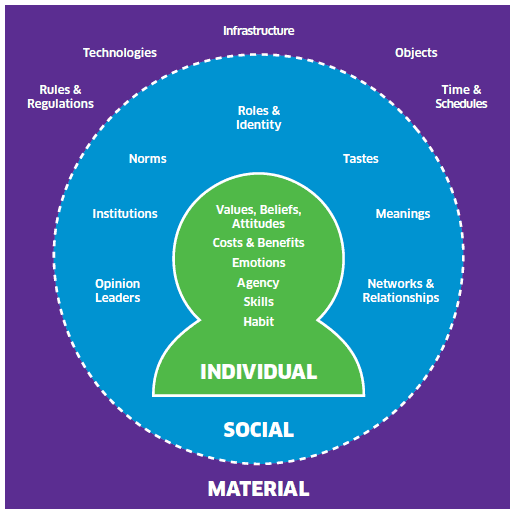
\includegraphics[width=0.5\linewidth]{figures/ism.png}
    \caption{Schematic diagram of the \ISM{} model of influences on behaviour}
    \label{fig:ism}
\end{figure}

\section{Scientists at the science-policy interface}\label{sec:litjust}

There is a significant body of research considering the nature of the \SPI{} and advising on the roles and practices that scientists should assume in order to engage with it. This work is frequently motivated by a recognition of the urgency of \CAN{} crises. Yet, much of the theorising about scientists' engagement at the \SPI{} does not admit the post-normal nature of \CAN{} crises and how this fundamentally transforms how policy decisions should be made. Further, with increasing numbers involved in \CAN-related advocacy, it is reasonable to suppose that ``scientists want to be more than chroniclers of a preventable tragedy'' (\cite{WyattGT2024}). However, indications from the literature are that climate researchers are not enlisting the advice about policy engagement that is available to them.

The existing advice on how scientists should engage at the \SPI{} begins from the perspective of policy, describes the needs of policymakers, and suggests how scientists can align to these needs. As such, this advice is using an \IDM-based approach to creating change in the behaviour of scientists. Behavioural Science suggests that influences other than lack of information is at play, and there is evidence that considerable tensions emerge for scientists who engage with policy. However, there has been little work to understand the perspectives and influences of scientists at the \SPI. 
